You are given a rooted binary tree with $n$ nodes (that is, each node has at most 2 children). Each node has a value attached to it. Given a query $k$, you are asked to count the number of simple paths whose values sum to exactly $k$.

For simplicity, we will consider a path to be valid in this context if it starts at some node and only moves down the tree. A path is not required to start at the root nor end at a leaf. For example, consider the following binary tree.

\begin{center}
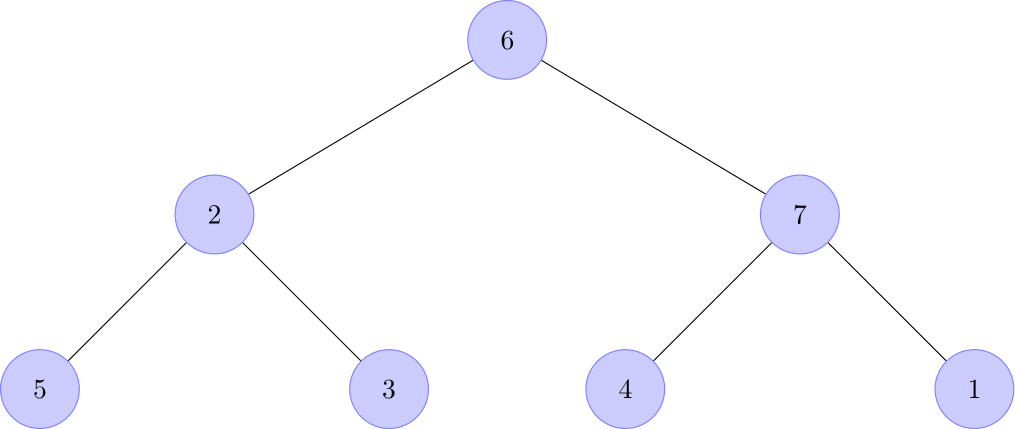
\includegraphics{example_binary_tree.png}
\end{center}

\textbf{6-2-3} would be considered a valid path, as would \textbf{6-7}, \textbf{2-5}, and even \textbf{4}. However, \textbf{4-7-1} is not a valid path because it goes up and then down. Nor would any paths which double back on themselves like \textbf{6-7-1-7}. We are also not considering the empty path to be valid.